\documentclass[review,3p,times]{elsarticle}

\usepackage{amsmath,amssymb,amsfonts}
\usepackage{graphicx}
\usepackage{booktabs}
\usepackage{multirow}
\usepackage{float}
\usepackage{algorithm}
\usepackage{algpseudocode}
\usepackage[colorlinks=true,citecolor=blue,linkcolor=blue,urlcolor=blue]{hyperref}

\journal{Advanced Engineering Informatics}

\newcommand{\breeze}{BREEZE}
\newcommand{\pucond}{N09\_M07\_F10}

\begin{document}
\begin{frontmatter}

\title{\breeze: A Training-Free Closed-Loop Physical-Gate Admission Framework
for LLM-Generated Bearing Fault Signals}

\author[a]{Author One}
\author[a]{Author Two}
\affiliation[a]{organization={Department}, city={City}, country={Country}}

\begin{abstract}
Large language models (LLMs) can synthesize condition-monitoring signals
without training a dedicated generative model, but prompt-level physical priors
remain open-loop. A generated window may enter the augmentation pool even when
its statistics, spectral energy, or envelope-spectrum structure are not
supported by the real training data for the requested fault class. This paper
proposes \breeze, a training-free closed-loop admission framework that wraps a
black-box generator with deterministic signal-processing gates calibrated only
on the real training split. The active gates check format legality, robust
time-statistic support, train-supported spectral shape, envelope-spectrum fault
evidence, reliability-gated current-sideband evidence, and diversity. Failed
generations are converted into structured reports for resampling; no waveform
repair or generator training is performed. On the Paderborn University
benchmark under the \pucond\ operating condition, the original $K{=}3$ closed
loop accepts 78.89\% of 450 generation slots with 2.05 LLM calls per slot. A
v2 verifier is evaluated as an offline rescreening of the same 450 slots: it
admits 286 slots, produces 761 accepted items before diversity, keeps 757
windows after diversity screening, and provides a more conservative
gate-compliance record. Compared with real-only training,
the v2 pool improves test accuracy by 14.33, 7.12, and 5.70 percentage points
for 10, 25, and 50 real windows per class, respectively; these three
comparisons remain significant after Benjamini--Hochberg correction over the
full family of 42 v2-vs-main-baseline paired tests. The v2 pool is competitive with, but does not uniformly
outperform, strong conventional augmentation and open-loop physics-guided
baselines. Experiments on a private four-channel machine-tool dataset are
reported as a schema-level verifier portability check, not as an augmentation
claim, because machine speed/geometry metadata and an audited synthetic pool
are unavailable. The results support train-calibrated physical-gate admission
as a practical and auditable way to control black-box synthetic data, while
also defining its empirical limits.
\end{abstract}

\begin{keyword}
Fault diagnosis \sep Large language model \sep Synthetic data \sep
Physics-based verification \sep Bearing \sep Training-free
\end{keyword}
\end{frontmatter}

\section{Introduction}
\label{sec:intro}

Fault data scarcity remains a bottleneck for intelligent condition monitoring.
Industrial machines rarely run to failure, controlled seeded-fault campaigns
are expensive, and fault-class imbalance is severe. Synthetic data therefore
play an important role in few-shot fault diagnosis, with methods ranging from
noise and geometric augmentation to variational autoencoders, generative
adversarial networks, and diffusion models~\cite{goodfellow,kingma,ho}.

LLM-based time-series synthesis offers a different route. A general-purpose
language model can be prompted to produce signal recipes or numeric sequences
conditioned on a machine state, avoiding the cost of training a new generator
for each dataset. The preceding MechaForge study showed that LLM-produced
signals can improve downstream fault diagnosis in low-data regimes, but it
also exposed a critical limitation: the generation process is open-loop. A
prompt may describe bearing physics, yet the emitted signal can still lack
class-consistent envelope-spectrum evidence, realistic impulsiveness, or
supported vibration-current structure before it enters the training pool.

Most existing physical approaches solve this problem at training time, by
embedding physics losses into a GAN, VAE, or diffusion objective. That is
powerful but not plug-and-play: a new machine, sensor configuration, or
closed-source generator requires re-training or re-design. Simple
post-generation filters are training-free but often stop at moment matching,
which misses diagnostic structure such as BPFO/BPFI alignment and resonance
band evidence. What is missing is an inference-time wrapper that can test a
candidate against train-calibrated diagnostic evidence, produce actionable
feedback, and admit only samples that pass the active gates, without modifying
the generator or repairing the waveform after the fact.

This paper proposes \breeze, a training-free closed-loop physical verification
framework. \breeze\ controls which generated samples are admitted into the
synthetic training pool. Its verifier is built from signal-processing and
bearing-diagnostic operations: robust train-split boundaries, Welch spectral
features, spectral-kurtosis-supported demodulation bands, Hilbert
envelope-spectrum checks, current sideband scores, and nearest-neighbour
diversity admission. All thresholds are calibrated from the real training
split only; the test set is never used for parameter selection. Failed samples
produce structured constraint reports that can be fed back to the generator
for at most $K$ resampling rounds. Samples that still fail are rejected rather
than locally corrected.

The word ``certificate'' is used in this manuscript only in the engineering
sense of an auditable gate-compliance record. It is not a formal proof of
physical correctness, distributional coverage, or downstream generalization.

The contributions are:
\begin{enumerate}
  \item A training-free, generator-agnostic physical-gate admission framework that
  wraps an existing LLM signal generator at inference time, using no generator
  retraining and no post-hoc waveform repair.
  \item A bearing-physics verifier with train-supported statistical,
  spectral, envelope, current-sideband, and diversity checks. Each admitted
  sample receives an auditable per-sample gate report.
  \item A v2 offline verifier design that reduces high-risk hard-band decisions using
  smooth spectral features, PSD-CDF Wasserstein distance, multi-band
  resonance support, and robust union domains. v2 is evaluated by rescreening
  the frozen $K{=}3$ generation pool, not by running a new v2 LLM loop.
  \item A reproducible evaluation protocol separating physical fidelity,
  admission cost, and downstream diagnostic utility on the Paderborn benchmark,
  plus schema-level verifier checks on additional PU operating conditions and a
  private four-channel machine-tool dataset.
\end{enumerate}

\section{Related Work}
\label{sec:related}

\subsection{Synthetic data for fault diagnosis}

Classical augmentation methods inject noise, rescale amplitudes, crop windows,
or mix samples. They are cheap and often strong baselines, as confirmed in
this study, but they cannot create new fault mechanisms. Trainable generative
models address this limitation by learning the real signal distribution:
GANs~\cite{goodfellow}, VAEs~\cite{kingma}, and diffusion
models~\cite{ho} have all been adapted to time-series augmentation. Sequence
generators such as C-RNN-GAN~\cite{mogren_crnngan}, recurrent conditional
GANs~\cite{esteban_rcgan}, and TimeGAN~\cite{timegan} explicitly model
temporal dynamics, while diffusion models such as TimeGrad~\cite{timegrad}
and CSDI~\cite{csdi} extend denoising or score-based generation to
multivariate time series.

For machinery diagnosis, generative augmentation is attractive because seeded
fault data are expensive and imbalanced. Conditional GAN/VAE/diffusion
pipelines can synthesize vibration windows for minority classes and have been
reported to improve classifiers in low-data regimes. These methods are the
closest family of competitors to \breeze, but they optimize the generator
itself. Therefore, their fidelity depends on architecture, training data,
loss weighting, and convergence. \breeze\ targets a different operating point:
it does not train or fine-tune the generator, and it asks whether generated
windows should be admitted after deterministic train-calibrated checks.

\subsection{Physics-informed generation and post-generation control}

Physics-informed learning embeds governing equations, conservation laws, or
domain penalties into model training~\cite{raissi_pinn}. In fault diagnosis,
the same principle motivates spectral, envelope, order-domain, or
kinematic-frequency losses for synthetic signals. Such constraints can produce
high-quality samples when the generator is trainable and the physical metadata
are available. However, they are less convenient for closed-source LLMs,
changing prompts, or private machines whose speed/geometry metadata are
incomplete.

Post-generation filtering is simpler: generate many candidates and reject
implausible ones. The risk is that generic filters often check only amplitudes
or low-order moments. \breeze\ can be viewed as train-calibrated rejection
sampling with diagnostic gates. Its novelty is not a formal physical proof;
it is the integration of bearing-specific envelope evidence, train-supported
spectral shape, reliability-gated current-sideband evidence, and diversity
admission into an auditable black-box generation wrapper.

\subsection{LLM-based signal generation and inference-time verification}

LLM-based synthesis reframes time-series generation as text-conditioned
reasoning or recipe generation. Its main appeal is zero-shot flexibility: a
black-box LLM can generate candidate waveforms without task-specific gradient
updates. Recent work has shown that language models can represent or forecast
time series when numerical sequences are serialized as text~\cite{llmtime},
and domain-specific LLM signal synthesis can use recipes or code-like
renderers rather than direct raw-number emission. Its weakness is that prompts
are not constraints. Inference-time verifier loops, including self-refinement
and rejection sampling, have become common in language tasks~\cite{madaan};
\breeze\ adapts this idea to machinery signals, replacing subjective LLM
self-critique with deterministic train-calibrated signal tests.

\subsection{Bearing diagnostics as generative verification}

Rolling-element faults excite structural resonances and modulate vibration at
kinematically determined characteristic frequencies. Envelope analysis and
spectral kurtosis are standard diagnostic tools for exposing these
signatures~\cite{randall,antoni,antoni_kurtogram}. Motor current signature
analysis (MCSA) provides complementary evidence through sidebands around the
electrical supply frequency~\cite{schoen}. \breeze\ uses these diagnostic
tools as admission gates: a generated window is not allowed into the training
pool unless the same signal-processing evidence expected from real data is
present in the candidate.

\section{Problem Formulation}
\label{sec:problem}

Let $\mathcal{D}_{\mathrm{tr}}=\{(x_i,y_i,m_i)\}$ denote real training
windows, where $x_i\in\mathbb{R}^{C\times N}$ is a multichannel signal,
$y_i$ is the class label, and $m_i$ contains available metadata such as speed
and load. A black-box generator $G$ proposes a candidate
$\tilde{x}_{r}\sim G(y,m,\phi_r)$ at feedback round $r$, where $\phi_r$ is
empty for the first attempt and becomes a constraint report after a rejection.
The goal is to construct a train-calibrated gate family
\begin{equation}
  \mathcal{G}_{y,m}=\{g_j(x;y,m,\mathcal{D}_{\mathrm{tr}})\}_{j=1}^{J},
  \qquad g_j\in\{0,1\},
\end{equation}
where every threshold used by $g_j$ is estimated from the training split only.
The gates are mixed predicates rather than a single type of one-sided
inequality:
\begin{equation}
\begin{aligned}
g_j(x)=1 \quad \Longleftrightarrow \quad
&a_j(y,m)\leq f_j(x)\leq b_j(y,m) && \text{for interval features,}\\
&f_j(x)\leq b_j(y,m)                  && \text{for upper-bound tests,}\\
&f_j(x)\geq a_j(y,m)                  && \text{for lower-bound evidence,}\\
&p_{\mathrm{fault}}(x)\leq b_h        && \text{for healthy fault-peak suppression,}\\
&d(e(x),\mathcal{S}_{y})\geq \delta_y && \text{for diversity admission.}
\end{aligned}
\end{equation}
Here $f_j$ denotes a deterministic signal feature, $p_{\mathrm{fault}}$ is an
envelope-spectrum fault-frequency prominence, $e(x)$ is the physical embedding
used for diversity, and $\mathcal{S}_{y}$ is the already admitted synthetic
set for class $y$. A candidate is admitted if it satisfies all active gates
before round $K$:
\begin{equation}
  \mathcal{S}_{K}=\{\tilde{x}: \exists r\leq K,\;\tilde{x}_r\in
  \mathcal{A}_{y,m}(\mathcal{S}_{y})\},\quad
  \mathcal{A}_{y,m}=\{x:g_j(x)=1,\;\forall j\in\mathcal{J}_{\mathrm{active}}\}.
\end{equation}
No learnable parameters are introduced in the verifier, and no test windows
are used during calibration. Membership in $\mathcal{A}_{y,m}$ is therefore a
gate-compliance statement, not a formal guarantee of physical validity or
future classifier performance.

\section{The \breeze\ Framework}
\label{sec:method}

\subsection{Overview}

Figure~\ref{fig:framework} summarizes the closed loop. A generator emits a
candidate signal or a parameter recipe that is rendered deterministically.
\breeze\ then executes four modules: M1 format/legality checks, M2 physical
feasible-set verification, M3 diversity admission, and M4 gate-report pool
logging. Failed gates are converted into a structured report containing the
violated feature, observed value, train-supported range, and an executable
instruction for the next generation attempt.

\begin{figure}[H]
\centering
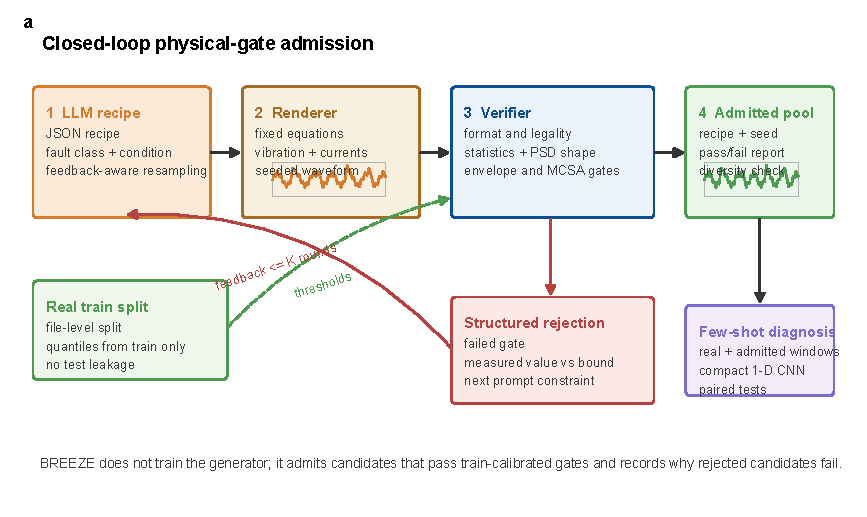
\includegraphics[width=\textwidth]{figs/framework.pdf}
\caption{The \breeze\ closed-loop physical-gate admission framework. The LLM
proposes a recipe, the renderer deterministically constructs a candidate
window, and the verifier admits or rejects it using gates calibrated only from
the real training split. Rejected candidates return structured feedback; passed
candidates enter a gate-admitted pool with an auditable report.}
\label{fig:framework}
\end{figure}

Figure~\ref{fig:boundary} makes the responsibility boundary explicit. The LLM
is responsible for proposing recipe fields, the renderer is responsible for the
signal equations, and the verifier is responsible only for train-calibrated
admission. This separation is important for the claims in this paper: a verifier
pass is not a proof that the LLM intrinsically understands fault physics.

\begin{figure}[H]
\centering
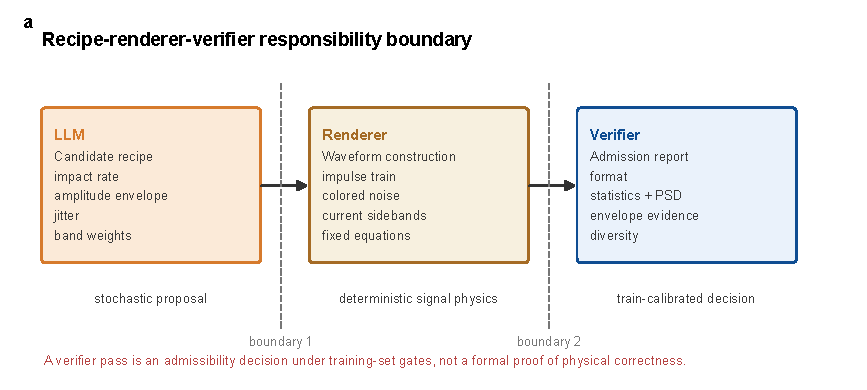
\includegraphics[width=\textwidth]{figs/responsibility_boundary.pdf}
\caption{Recipe-renderer-verifier responsibility boundary. The stochastic LLM
proposal, deterministic signal construction, and train-calibrated gate decision
are separate components. The verifier can reject and report constraint
violations, but it does not repair a waveform or provide a formal physical
correctness certificate.}
\label{fig:boundary}
\end{figure}

\subsection{M1: format and legality}

M1 rejects malformed outputs: wrong shape, non-finite values, near-constant
channels, and long repeated segments. In the PU study the expected shape is
$(3,2048)$ after selecting one vibration channel and two phase-current
channels. In the private machine-tool study the schema is $(4,2048)$ for
three vibration axes plus current.

\subsection{M2: physical feasible-set gates}

\paragraph{Boundary-restricted statistics.}
For each class and channel, \breeze\ estimates train-split quantile intervals
for RMS, peak value, standard deviation, kurtosis, skewness, and crest factor.
The original verifier uses per-feature intervals. The v2 verifier uses a union
domain: a candidate passes if it lies inside either the legacy quantile box or
a robust axis ellipsoid defined by median/IQR-standardized feature distances.
This prevents a physically plausible candidate from being rejected solely
because one correlated statistic is slightly outside a marginal boundary.

\paragraph{Spectral shape and PSD distance.}
The original verifier uses hard Welch-PSD band fractions. v2 replaces this
with overlapping triangular bands and a normalized PSD-CDF Wasserstein-1
distance to the class train reference. These features are still deterministic
and train-calibrated, but they avoid discontinuities when a spectral peak lies
near a hard band boundary.

\paragraph{Envelope-spectrum evidence.}
For fault classes, the vibration signal is band-passed through train-supported
resonance bands, demodulated using the Hilbert transform, and checked for a
prominent peak near the class characteristic frequency. Healthy candidates
must not display a fault-frequency envelope peak above the healthy threshold.
v2 uses the top three train-supported resonance bands instead of a single
spectral-kurtosis maximum.

\paragraph{Current-sideband evidence.}
For the PU setting, two phase-current channels are combined into a
vector-current MCSA score. If the train split shows that sidebands are not
separable from healthy current spectra, the MCSA score is recorded in the
gate report but not used as a hard gate. This avoids enforcing a constraint
that the real train data do not support.

\subsection{M3: diversity admission}

The admitted pool should not be a set of near-duplicates. \breeze\ computes a
physical embedding from statistics, spectral fractions, envelope scores, and
current-sideband features. Candidate windows whose nearest-neighbour distance
to the accepted pool is below a class-wise real-real reference threshold are
not admitted. The threshold is derived from the train split.

\subsection{M4: gate-report resampling}

Algorithm~\ref{alg:loop} defines the closed loop. The verifier never repairs a
failed waveform. It either admits the generated candidate as-is with a
gate-compliance report, or rejects it and returns a report to guide another generator
call.

\begin{algorithm}
\caption{\breeze\ closed-loop physical-gate admission}
\label{alg:loop}
\begin{algorithmic}[1]
\Require class $y$, metadata $m$, generator $G$, verifier $\mathcal{V}$,
maximum feedback rounds $K$
\State $\phi_0 \gets \varnothing$
\For{$r=0$ to $K$}
  \State $\tilde{x}_r \sim G(y,m,\phi_r)$
  \State $(p_r,R_r)\gets\mathcal{V}(\tilde{x}_r,y,m)$
  \If{$p_r=1$}
    \State \Return admitted sample and gate report $R_r$
  \EndIf
  \State $\phi_{r+1}\gets\mathrm{ReportToFeedback}(R_r)$
\EndFor
\State \Return rejection
\end{algorithmic}
\end{algorithm}

\section{Experimental Setup}
\label{sec:setup}

\subsection{Paderborn benchmark}

The main benchmark is the Paderborn University bearing dataset~\cite{lessmeier}
under condition \pucond\ (900 rpm, 0.7 Nm torque, 1000 N radial load). Raw
64 kHz signals are decimated to 8 kHz using zero-phase FIR filtering. Windows
have 2048 samples. The retained channels are `vibration\_1',
`phase\_current\_1', and `phase\_current\_2'; internal short names
`X/Y/Z' refer to these retained channels and should not be interpreted as
three-axis PU vibration. The file-based split uses the first 80\% of
measurement files for training and the last 20\% for testing for every
bearing. It contains 3846 train windows and 962 test windows, with no file-ID
overlap.

\begin{table}[H]
\centering
\caption{PU file-split window counts under \pucond.}
\label{tab:pu_split}
\begin{tabular}{lrrrr}
\toprule
Split & healthy & OR & IR & total \\
\midrule
Train & 1200 & 1202 & 1444 & 3846 \\
Test  & 300  & 301  & 361  & 962 \\
\bottomrule
\end{tabular}
\end{table}

\subsection{Private machine-tool dataset}

A private laboratory machine-tool dataset is used to test schema-level
verifier portability.
Internal documentation describes a CNC machining acquisition system driven by a
standardized G-code process. The signals are collected by an NI acquisition card
at 4 kHz with four synchronous analog channels: $X/Y/Z$ vibration and spindle
load Current. The documented dataset covers normal machining, lead-screw
anomaly, and base imbalance. In the present BREEZE workspace, however, local
file names identify three classes only as 1, 2, and 3, and the available
documentation does not unambiguously map these prefixes to the physical state
names. We therefore report them as MT-1, MT-2, and MT-3. The BREEZE windows
have 2048 samples with stride 1024, corresponding to 0.512 s windows and
0.256 s hops at 4 kHz. Train files are 1, 2, 4, 5, and 10; test files are 7
and 8. Because machine geometry, operating speed, and the prefix-to-state
mapping are unavailable in the audited workspace metadata, the machine-tool
verifier uses only generic train-calibrated statistics and normalized spectral
constraints.

\subsection{Baselines and classifier}

The PU downstream study compares real-only training, noise augmentation, VAE
and GAN baselines, few-shot VAE/GAN baselines, open-loop basic LLM generation,
open-loop physics-guided generation, stats-only filtering, envelope-only
filtering, the original \breeze\ pools for $K=0,1,2,3$, and the v2
offline-rescreened pool. The classifier is a compact 1D CNN trained for 60 epochs. Few-shot
settings use 10, 25, or 50 real windows per class and eight random seeds.
Synthetic pools are capped at 200 windows per class when added to a few-shot
training set. Accuracy, macro-F1, per-class F1 where available, physical MMD,
nearest-neighbour diversity, acceptance rate, and paired Wilcoxon tests are
reported. The v2 pool is not a new v2 LLM generation run; it is a stricter
offline rescreening of the frozen original $K{=}3$ generated candidates.

\section{Results}
\label{sec:results}

\subsection{Closed-loop acceptance}

The original physics-guided closed loop generated 450 slots. Here a slot means
one requested LLM generation unit for a class. A feasible slot may contribute
the selected round window and zero or more feasible expansion windows produced
from the same slot recipe. As $K$ increases,
the accepted-slot rate rises while the average number of LLM calls remains
near two at $K=3$ (Table~\ref{tab:acceptance}). The v2 offline rescreening is
stricter: it admits 286 of 450 slots, produces 761 accepted items before
diversity, keeps 757 generated windows after diversity, and yields class
counts 192/304/261 for healthy/OR/IR. Since v2 does not call the LLM again,
the LLM-call cost in Table~\ref{tab:acceptance} belongs only to the original
closed-loop run.

\begin{table}[H]
\centering
\caption{Closed-loop acceptance and cost for the original physics-guided run.}
\label{tab:acceptance}
\begin{tabular}{rrrr}
\toprule
$K$ & accepted slots & acceptance & mean LLM calls/slot \\
\midrule
0 & 253/450 & 0.5622 & 1.0000 \\
1 & 295/450 & 0.6556 & 1.4378 \\
2 & 330/450 & 0.7333 & 1.7822 \\
3 & 355/450 & 0.7889 & 2.0489 \\
\bottomrule
\end{tabular}
\end{table}

Table~\ref{tab:v2_fail} and Figure~\ref{fig:failure} summarize why v2 rejects terminal slots. Counts can
exceed the number of rejected slots because one terminal candidate may violate
multiple gates. Healthy rejections are dominated by forbidden fault-frequency
envelope peaks, while OR/IR rejections are dominated by the statistical union
domain and soft spectral shape. This failure pattern is useful for diagnosing
which parts of the LLM recipe family remain weak; it should not be interpreted
as a guarantee that all passed samples are physically correct.

\begin{table}[H]
\centering
\caption{Terminal rejected-slot failure counts in v2 offline rescreening.}
\label{tab:v2_fail}
\begin{tabular}{lrrrr}
\toprule
Class & rejected slots & stats & soft spectrum & envelope / PSD-W1 \\
\midrule
healthy & 60 & 4 & 0 & 51 / 10 \\
OR      & 60 & 45 & 21 & 0 / 0 \\
IR      & 44 & 43 & 7 & 0 / 0 \\
\bottomrule
\end{tabular}
\end{table}

\begin{figure}[H]
\centering
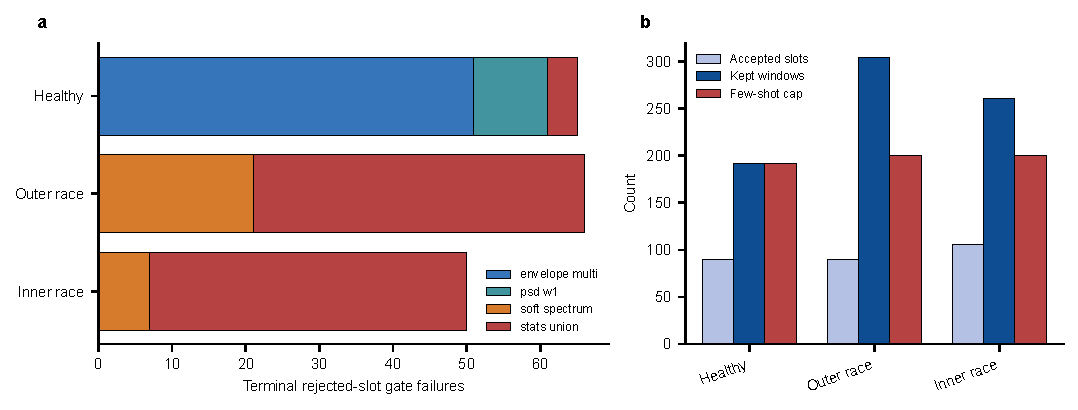
\includegraphics[width=\textwidth]{figs/failure_reasons.pdf}
\caption{Failure and slot-window accounting for v2 offline rescreening. Panel a
shows terminal rejected-slot gate failures by class. Panel b shows how accepted
slots expand into kept windows and the 200-window/class few-shot cap. Source
data are the v2 fail-reason and slot-window mapping CSV files.}
\label{fig:failure}
\end{figure}

Figure~\ref{fig:failure_case} gives a concrete rejected candidate from the same
audit trail. The slot is labelled healthy by the generator output, but its
envelope spectrum contains forbidden IR-frequency evidence above the
train-calibrated healthy limit. This is a single diagnostic example, not a
distributional result; the aggregate failure counts are reported in
Table~\ref{tab:v2_fail}.

\begin{figure}[H]
\centering
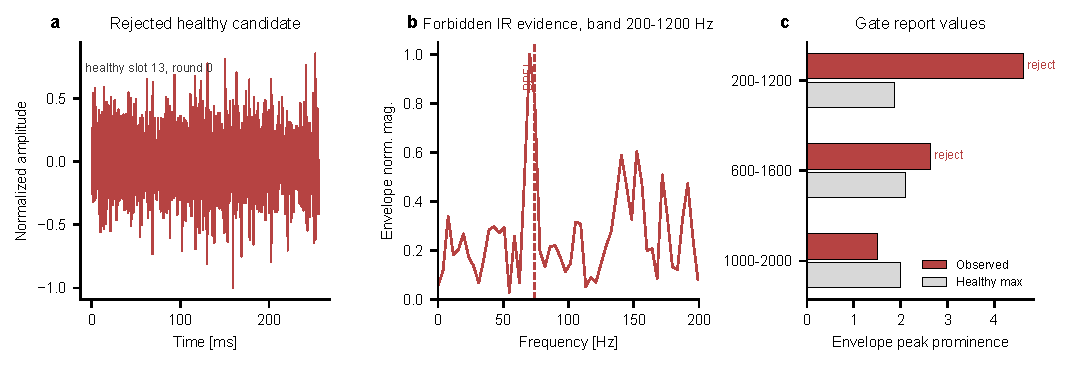
\includegraphics[width=\textwidth]{figs/failure_case.pdf}
\caption{Example of a rejected healthy candidate. Panel a shows the candidate
waveform. Panel b shows the envelope spectrum in the resonance band that
triggered forbidden IR-frequency evidence. Panel c reports the observed
envelope peak prominence against the train-calibrated healthy upper limit for
the three IR resonance bands. The source record is
\texttt{runs/rescreen\_v2\_full/records/healthy\_0013.json}.}
\label{fig:failure_case}
\end{figure}

\subsection{Coverage sensitivity}

Table~\ref{tab:coverage} reports train/test pass rates for v1 verifier
coverages c85, c90, and c95. Pass rates change modestly because the hard
spectrum gate is unchanged across these calibrations; this motivated the v2
smooth-spectrum and PSD-W1 redesign.

\begin{table}[H]
\centering
\caption{PU verifier coverage sensitivity. Rates are recomputed on frozen
train/test splits; thresholds are calibrated without using test data.}
\label{tab:coverage}
\begin{tabular}{llrrrrr}
\toprule
Coverage & split & all & healthy & OR & IR & spectrum fails \\
\midrule
c85 & train & 0.9285 & 0.9300 & 0.9285 & 0.9273 & 104 \\
c85 & test  & 0.8992 & 0.9100 & 0.8970 & 0.8920 & 44 \\
c90 & train & 0.9368 & 0.9425 & 0.9326 & 0.9356 & 104 \\
c90 & test  & 0.9148 & 0.9400 & 0.9103 & 0.8975 & 44 \\
c95 & train & 0.9441 & 0.9467 & 0.9443 & 0.9418 & 104 \\
c95 & test  & 0.9210 & 0.9400 & 0.9169 & 0.9086 & 44 \\
\bottomrule
\end{tabular}
\end{table}

\subsection{Physical fidelity and diversity}

Figure~\ref{fig:waves} compares real and gate-admitted synthetic examples in
time, FFT, and envelope-spectrum domains. Figure~\ref{fig:box} shows the effect
of admission on RMS and kurtosis distributions. Figure~\ref{fig:metrics} and
Table~\ref{tab:phys} summarize feature-MMD and nearest-neighbour diversity.
MMD2 is computed on an eight-dimensional
vibration-channel feature vector: RMS, kurtosis, crest factor, skewness, and
Welch-PSD band-energy fractions over 0--500, 500--1500, 1500--2500, and
2500--4000 Hz. For each class, up to 150 synthetic windows and 150 train-real
windows are standardized by the sampled real mean and standard deviation, and
RBF-kernel MMD2 is computed with the median pairwise-distance bandwidth
heuristic. v2 improves MMD over the original \breeze\ $K=3$
pool for OR and IR, but not for healthy. Open-loop physics-guided and
envelope-only pools remain competitive on this particular feature-MMD metric,
so physical-gate admission should be interpreted jointly with gate reports and
downstream utility rather than as a universal MMD minimizer.

\begin{figure}[H]
\centering
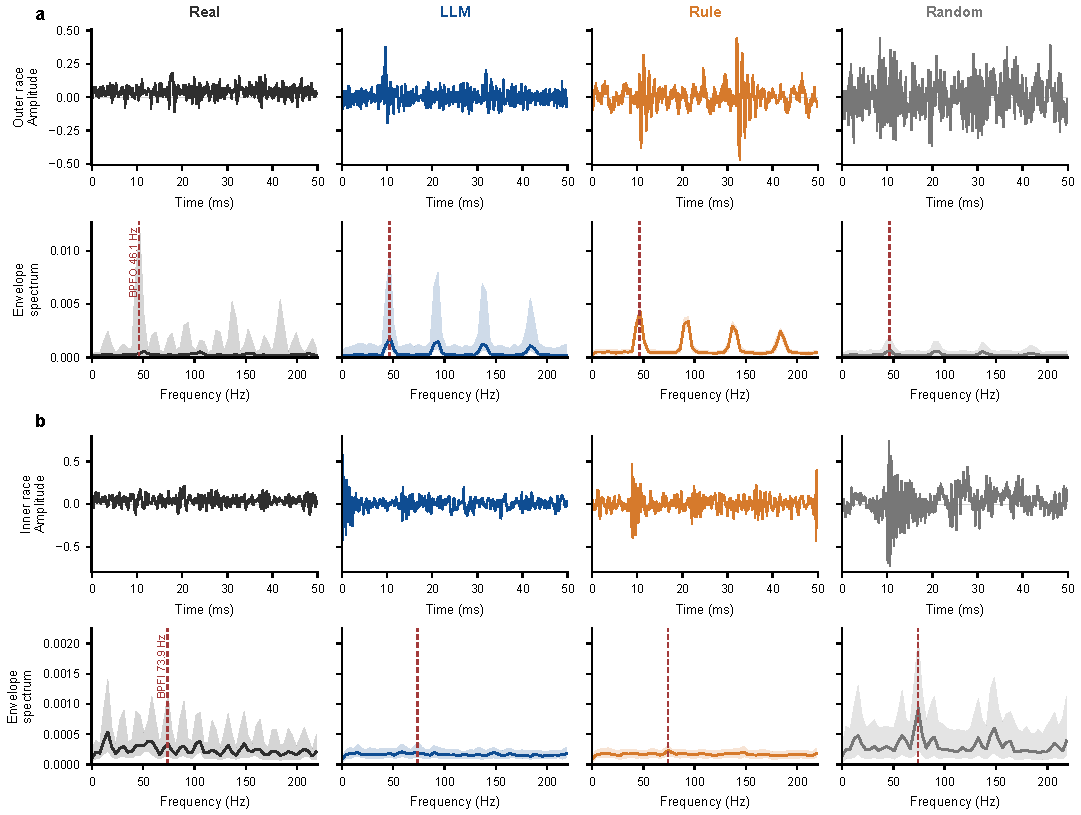
\includegraphics[width=\textwidth]{figs/waveforms.pdf}
\caption{Representative real and v2 gate-admitted synthetic windows in the
time, FFT, and envelope-spectrum domains. Blue traces denote real train windows
and orange traces denote admitted synthetic windows. Vertical reference lines
mark BPFO and BPFI; the class-relevant fault frequency is highlighted in red.}
\label{fig:waves}
\end{figure}

\begin{figure}[H]
\centering
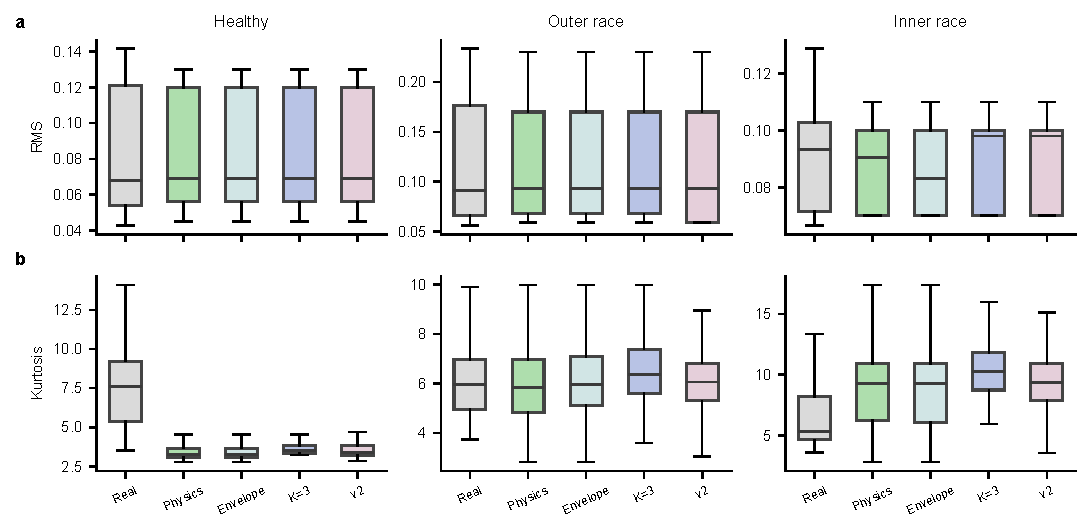
\includegraphics[width=\textwidth]{figs/boxplots.pdf}
\caption{RMS and kurtosis distributions for real windows and synthetic pools.
The v2 pool is included when available.}
\label{fig:box}
\end{figure}

\begin{figure}[H]
\centering
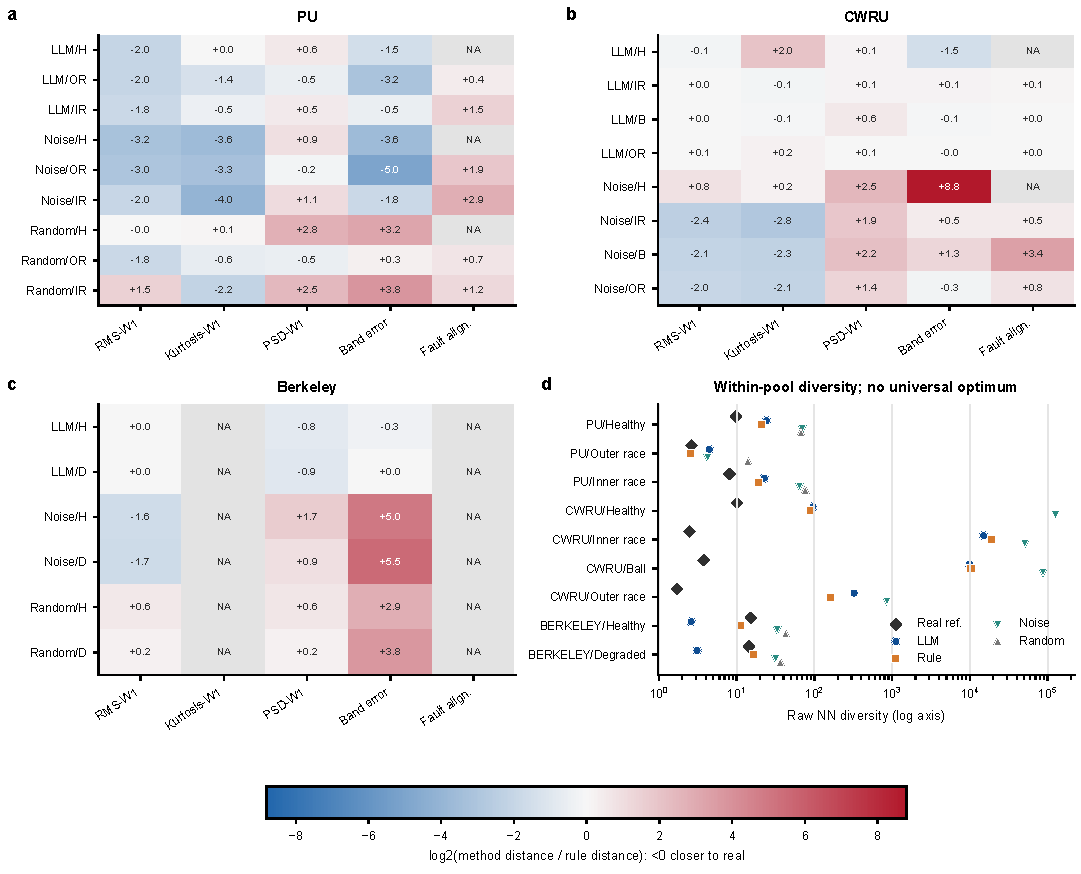
\includegraphics[width=\textwidth]{figs/metric_distances.pdf}
\caption{Feature-distance and diversity summaries for synthetic pools. Panel a
reports MMD2 on standardized eight-dimensional vibration features. Panel b
reports nearest-neighbour diversity normalized by the corresponding real-real
reference. Lower MMD2 is closer to the sampled real feature distribution; a
diversity ratio near one indicates real-like spacing under this feature set.}
\label{fig:metrics}
\end{figure}

\begin{table}[H]
\centering
\caption{Physical fidelity and diversity. Lower MMD2 is closer to real
features; NN diversity should be interpreted relative to the real-real
reference.}
\label{tab:phys}
\begin{tabular}{llrrrr}
\toprule
Pool & class & $n$ & MMD2 & NN div. & real NN div. \\
\midrule
open-loop basic & healthy & 135 & 0.7769 & 1.3263 & 0.8910 \\
open-loop basic & OR & 142 & 1.2786 & 0.7972 & 0.4122 \\
open-loop basic & IR & 139 & 1.5248 & 1.6169 & 0.8598 \\
open-loop phys. & healthy & 150 & 0.1481 & 0.3495 & 0.8910 \\
open-loop phys. & OR & 150 & 0.0451 & 0.4224 & 0.4122 \\
open-loop phys. & IR & 150 & 0.0829 & 0.7162 & 0.8598 \\
\breeze\ $K=3$ & healthy & 519 & 0.1378 & 0.3305 & 0.8910 \\
\breeze\ $K=3$ & OR & 638 & 0.0776 & 0.4239 & 0.4122 \\
\breeze\ $K=3$ & IR & 390 & 0.1990 & 0.6919 & 0.8598 \\
\breeze\ v2 & healthy & 192 & 0.1507 & 0.3468 & 0.8910 \\
\breeze\ v2 & OR & 304 & 0.0713 & 0.4212 & 0.4122 \\
\breeze\ v2 & IR & 261 & 0.1254 & 0.7123 & 0.8598 \\
\bottomrule
\end{tabular}
\end{table}

\subsection{Downstream few-shot diagnosis}

Figure~\ref{fig:downstream} and Table~\ref{tab:downstream} report downstream
accuracy. The v2 offline-rescreened pool outperforms real-only training in all
three few-shot regimes, and these three comparisons remain significant after
Benjamini--Hochberg correction across the full family of 42
v2-vs-main-baseline paired tests. However, v2 is
not uniformly higher than all conventional baselines: envelope-only is higher
at 10-shot, open-loop physics-guided and noise augmentation are higher at
25-shot, and noise augmentation is strongest at 50-shot in the frozen main
table. This is an important boundary of the current evidence.

\begin{figure}[H]
\centering
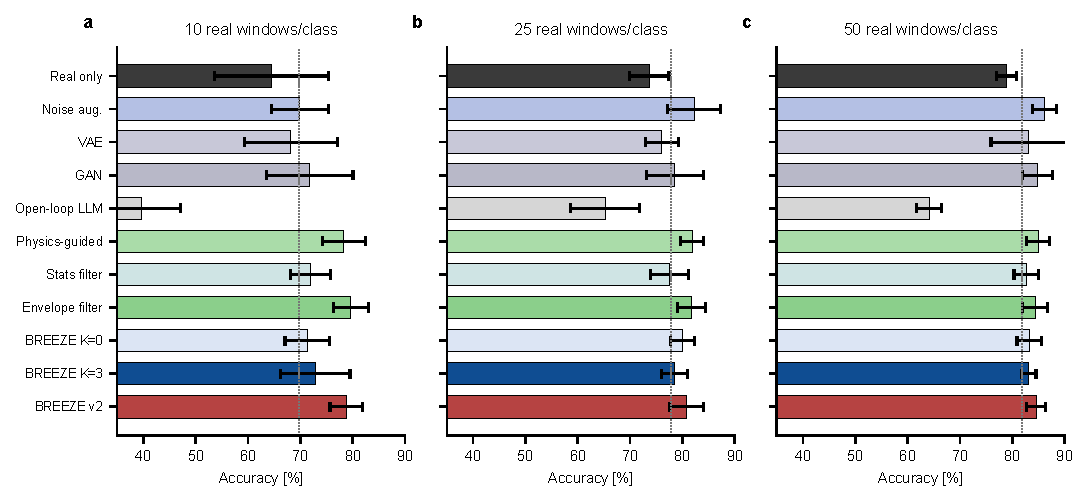
\includegraphics[width=\textwidth]{figs/downstream_bars.pdf}
\caption{Downstream test accuracy for selected baselines. The final bar shows
the v2 offline-rescreened pool when the v2 evaluation file is present.}
\label{fig:downstream}
\end{figure}

\begin{table}[H]
\centering
\caption{Selected PU downstream results. Values are mean $\pm$ standard
deviation over eight seeds. The v2 pool uses the 200-window/class synthetic
cap, giving 192+200+200=592 synthetic windows in each few-shot run.}
\label{tab:downstream}
\begin{tabular}{llccc}
\toprule
Baseline & Metric & 10/class & 25/class & 50/class \\
\midrule
real only & Acc. & $0.6447\pm0.1085$ & $0.7370\pm0.0374$ & $0.7886\pm0.0195$ \\
open-loop phys. & Acc. & $0.7834\pm0.0408$ & $0.8186\pm0.0221$ & $0.8498\pm0.0219$ \\
envelope-only & Acc. & $0.7964\pm0.0337$ & $0.8180\pm0.0267$ & $0.8439\pm0.0238$ \\
noise aug. & Acc. & $0.6992\pm0.0544$ & $0.8225\pm0.0508$ & $0.8616\pm0.0235$ \\
\breeze\ $K=3$ & Acc. & $0.7283\pm0.0667$ & $0.7844\pm0.0247$ & $0.8317\pm0.0138$ \\
\breeze\ v2 & Acc. & $0.7880\pm0.0312$ & $0.8082\pm0.0324$ & $0.8456\pm0.0174$ \\
\midrule
real only & Macro-F1 & $0.6040\pm0.1292$ & $0.7184\pm0.0425$ & $0.7743\pm0.0253$ \\
\breeze\ v2 & Macro-F1 & $0.7906\pm0.0289$ & $0.8079\pm0.0354$ & $0.8484\pm0.0178$ \\
\bottomrule
\end{tabular}
\end{table}

\begin{table}[H]
\centering
\caption{Selected paired Wilcoxon tests on accuracy for \breeze\ v2. The $q$
column is Benjamini--Hochberg adjusted across the full family of 42
v2-vs-main-baseline tests; the complete table is provided in the revision
statistics output.}
\label{tab:wilcoxon}
\begin{tabular}{llrrr}
\toprule
Comparison & n/class & Delta & $p$ & $q$ \\
\midrule
v2 vs real only & 10 & +0.1433 & 0.0078 & 0.0328 \\
v2 vs real only & 25 & +0.0712 & 0.0156 & 0.0438 \\
v2 vs real only & 50 & +0.0570 & 0.0078 & 0.0328 \\
v2 vs \breeze\ $K=3$ & 10 & +0.0597 & 0.0156 & 0.0438 \\
v2 vs \breeze\ $K=3$ & 25 & +0.0238 & 0.0547 & 0.1209 \\
v2 vs \breeze\ $K=3$ & 50 & +0.0139 & 0.0391 & 0.0965 \\
v2 vs envelope-only & 10 & -0.0084 & 0.2109 & 0.3281 \\
v2 vs open-loop phys. & 25 & -0.0104 & 0.7422 & 0.8203 \\
v2 vs noise aug. & 50 & -0.0160 & 0.1484 & 0.2494 \\
\bottomrule
\end{tabular}
\end{table}

\subsection{Feedback-round ablation}

Figure~\ref{fig:k} shows the acceptance-cost trade-off and the downstream
accuracy of the original \breeze\ $K=0,\ldots,3$ pools. Increasing $K$ raises
admission probability, but downstream accuracy is not monotonic. This supports
the paper's central distinction: physical admission and diagnostic utility
must be evaluated separately.

\begin{figure}[H]
\centering
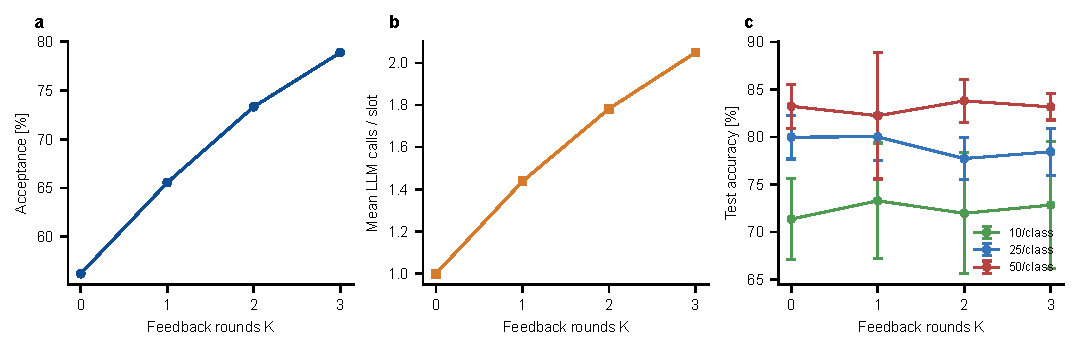
\includegraphics[width=\textwidth]{figs/acceptance_k.pdf}
\caption{Original closed-loop acceptance, average LLM calls, and downstream
accuracy across feedback rounds $K$.}
\label{fig:k}
\end{figure}

\subsection{PU cross-condition verifier audit}

To address operating-condition dependence without inventing an unrun
cross-condition LLM experiment, we also instantiate the v2 verifier separately
on all four preprocessed PU conditions and evaluate real train/test pass rates.
Figure~\ref{fig:cross_condition_heatmap} and Table~\ref{tab:cross_condition}
report compact class-group summaries. This is
a verifier coverage audit only: no synthetic pool is generated for these extra
conditions. The results show that fault-class windows generally remain within
the train-calibrated gates, while the healthy class is conservatively rejected
more often because the forbidden fault-frequency envelope gate is strict.

\begin{figure}[H]
\centering
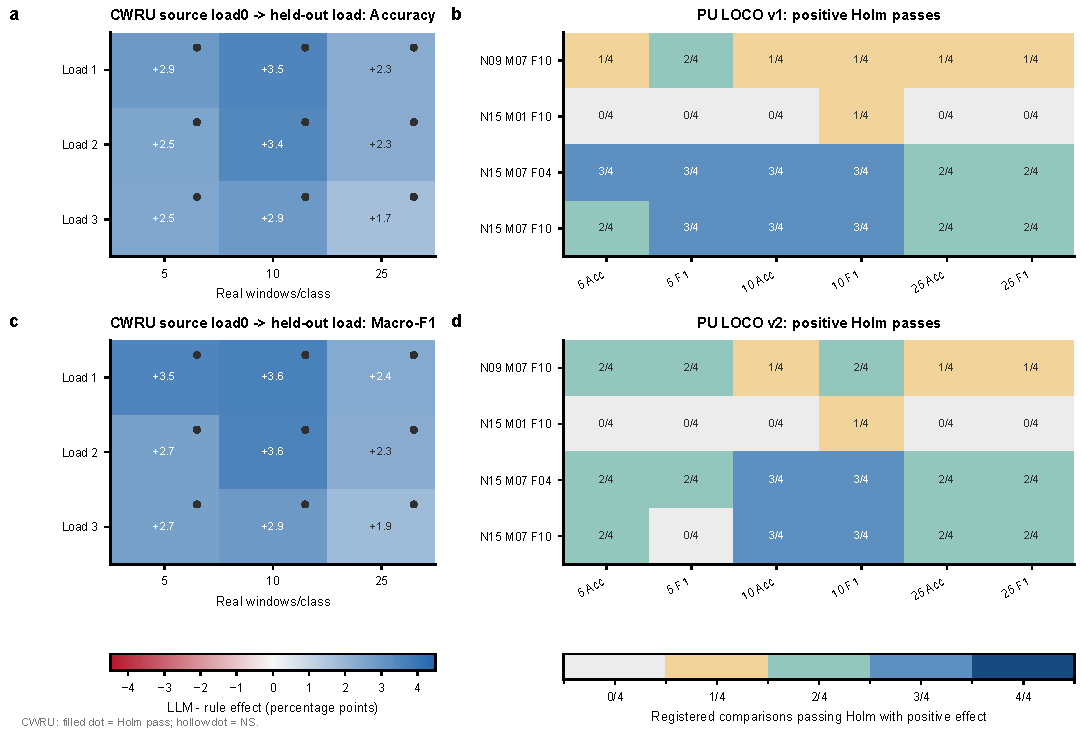
\includegraphics[width=\textwidth]{figs/cross_condition_heatmap.pdf}
\caption{PU cross-condition v2 verifier audit. Heatmaps show train and test
pass rates after recalibrating the verifier within each condition. This figure
audits gate coverage on real windows only and does not report cross-condition
synthetic augmentation.}
\label{fig:cross_condition_heatmap}
\end{figure}

\begin{table}[H]
\centering
\caption{PU cross-condition v2 verifier audit. Fault mean is the average of OR
and IR pass rates. The audit is not a cross-condition augmentation experiment.}
\label{tab:cross_condition}
\begin{tabular}{lrrrr}
\toprule
Condition & train healthy & train fault mean & test healthy & test fault mean \\
\midrule
N09\_M07\_F10 & 0.7125 & 0.9507 & 0.6800 & 0.8729 \\
N15\_M01\_F10 & 0.7049 & 0.9533 & 0.6967 & 0.9428 \\
N15\_M07\_F04 & 0.6938 & 0.9595 & 0.7667 & 0.9433 \\
N15\_M07\_F10 & 0.6958 & 0.9516 & 0.6777 & 0.8545 \\
\bottomrule
\end{tabular}
\end{table}

\subsection{Private machine-tool schema audit}

Table~\ref{tab:mt} summarizes the private dataset. The four-channel verifier
uses normalized PSD features rather than PU bearing kinematics. The sampling
rate is known to be 4 kHz, but absolute machine-order gates are not used because
the workspace lacks the corresponding operating-speed and geometry metadata.
Train pass rates are 0.938--0.959. Test pass rates reveal distribution shift in
MT-1 and MT-3, especially test file 1\_7; this is useful diagnostic information
rather than a result to hide. Real-only downstream accuracy rises from
$0.3431\pm0.0321$ at 10 real windows per class to $0.7006\pm0.0626$ at 50
real windows per class. No machine-tool synthetic pool has been generated and
screened yet, so no augmentation gain is claimed on this dataset.

\begin{table}[H]
\centering
\caption{Private machine-tool results. The documented dataset contains normal
machining, lead-screw anomaly, and base imbalance, but labels are reported
anonymously because the local files do not map prefixes 1/2/3 to those physical
state names.}
\label{tab:mt}
\begin{tabular}{llrrr}
\toprule
Block & class/setting & $n$ & pass or Acc. & macro-F1 \\
\midrule
Verifier train & MT-1 & 675 & 0.9585 & -- \\
Verifier train & MT-2 & 383 & 0.9530 & -- \\
Verifier train & MT-3 & 679 & 0.9381 & -- \\
Verifier test & MT-1 & 166 & 0.7590 & -- \\
Verifier test & MT-2 & 166 & 0.9337 & -- \\
Verifier test & MT-3 & 154 & 0.7727 & -- \\
Real-only 10/class & all & 8 seeds & $0.3431\pm0.0321$ & $0.3368\pm0.0318$ \\
Real-only 25/class & all & 8 seeds & $0.4964\pm0.0566$ & $0.4897\pm0.0530$ \\
Real-only 50/class & all & 8 seeds & $0.7006\pm0.0626$ & $0.7021\pm0.0632$ \\
\bottomrule
\end{tabular}
\end{table}

\section{Discussion}
\label{sec:discussion}

\paragraph{Why physical-gate admission rather than generator training?}
\breeze\ is useful when the generator is expensive, closed source, or expected
to change. The verifier is deterministic and calibrated from the train split;
therefore, the same admission logic can wrap an LLM recipe generator today and
a different black-box generator later.

\paragraph{Physical fidelity is not identical to downstream accuracy.}
The experiments show that gate-admitted pools can improve real-only diagnosis
and the original \breeze\ baseline in low-data settings, but strong
conventional augmentation can still win in some higher-shot regimes. This does
not invalidate physical-gate admission; it clarifies the contribution.
\breeze\ provides auditable control over which generated samples are admitted,
not a guarantee that physical filtering alone will dominate every
classifier-training baseline.

\paragraph{Threshold calibration.}
All thresholds are train-only. The c85/c90/c95 sensitivity study shows modest
changes in real pass rates and exposes a hard-spectrum limitation in the v1
verifier. The v2 redesign addresses this through smooth spectral features and
PSD-W1. The additional four-condition PU audit shows that v2 can be calibrated
under multiple operating conditions, but it also exposes a conservative healthy
fault-peak suppression gate. Therefore, a full cross-condition augmentation
claim still requires new generated pools and downstream evaluation.

\paragraph{Circular validation risk.}
The verifier and the deterministic renderer both use bearing-domain concepts.
This raises a possible circular-validation risk: a generator may learn to
satisfy the measured gates without matching all aspects of the real fault
distribution. We reduce this risk by reporting downstream diagnosis, MMD,
diversity, pass/fail records, and strong augmentation baselines, but external
physical validation and human diagnostic review remain necessary before
industrial deployment.

\paragraph{Limitations.}
The current PU results focus on one operating condition. The private
machine-tool study verifies schema-level portability, but not augmentation,
because no audited private synthetic pool exists yet. The class semantics of
the private data must be provided before physical fault names can be written.
The current downstream study uses a compact 1D CNN; additional classifiers are
needed to test model-level robustness. Finally, exact citation metadata for
unpublished or in-house MechaForge assets must be completed before submission.

\section{Conclusion}
\label{sec:conclusion}

This paper introduced \breeze, a training-free closed-loop framework for
physical-gate admission of LLM-generated fault-diagnosis signals. Instead of
training a new generator or repairing failed waveforms, \breeze\ tests each
candidate against train-calibrated signal-processing gates, feeds structured
failure reports back for resampling, and admits only samples with auditable
gate reports. On the Paderborn benchmark, the v2 offline-rescreened pool
improves few-shot real-only diagnosis after multiple-test correction, while
physical metrics and strong baselines reveal where the method is competitive
rather than dominant. Additional PU operating-condition audits and the private
machine-tool study show how the verifier can be reconfigured, but not yet that
synthetic augmentation transfers across all machines and conditions. Future
work will add full cross-speed/load generation loops, audited synthetic pools
for the private dataset, additional diagnostic classifiers, and broader
comparisons with trainable physics-informed generators.

\section*{Reproducibility Notes}

The numerical results in this manuscript are traceable to the following local
outputs:
\begin{itemize}
  \item \texttt{results/downstream\_file.csv}
  \item \texttt{results/custom\_pool\_eval.csv}
  \item \texttt{results/pool\_metrics.csv} and
  \texttt{results/pool\_metrics\_v2.csv}
  \item \texttt{results/calibration\_sensitivity.csv}
  \item \texttt{results/revision\_v2\_significance\_all\_baselines\_bh.csv}
  \item \texttt{results/revision\_v2\_slot\_window\_mapping.csv}
  \item \texttt{results/revision\_v2\_rejected\_slot\_fail\_reasons.csv}
  \item \texttt{results/cross\_condition\_verifier\_full.csv}
  \item \texttt{results/mt\_verifier\_real\_pass.csv}
  \item \texttt{results/mt\_real\_only\_eval.csv}
\end{itemize}
Snapshot reports are stored in the project \texttt{reports/} directory.

\section*{Data Availability Statement}

The Paderborn University bearing dataset is publicly available from the data
provider. The private machine-tool dataset contains laboratory data and is not
publicly released in the current submission; derived aggregate metrics,
verifier summaries, and split descriptions are provided in the supplementary
material. Code, prompts, gate reports, and result tables can be shared subject
to institutional and data-use constraints.

\section*{Declaration of Generative AI and AI-Assisted Technologies in the
Manuscript Preparation Process}

During the preparation of this work, the authors used OpenAI Codex to assist
with code inspection, experiment scripting, result-table assembly, figure
generation, and manuscript drafting. After using this tool, the authors
reviewed, verified, and edited the content and take full responsibility for
the final manuscript.

\bibliographystyle{elsarticle-num}
\begin{thebibliography}{00}

\bibitem{goodfellow}
I. Goodfellow, J. Pouget-Abadie, M. Mirza, B. Xu, D. Warde-Farley,
S. Ozair, A. Courville, Y. Bengio, Generative adversarial nets, in:
Advances in Neural Information Processing Systems, 2014.

\bibitem{kingma}
D. P. Kingma, M. Welling, Auto-encoding variational Bayes, in:
International Conference on Learning Representations, 2014.

\bibitem{ho}
J. Ho, A. Jain, P. Abbeel, Denoising diffusion probabilistic models, in:
Advances in Neural Information Processing Systems, 2020.

\bibitem{mogren_crnngan}
O. Mogren, C-RNN-GAN: continuous recurrent neural networks with adversarial
training, arXiv:1611.09904, 2016.

\bibitem{esteban_rcgan}
C. Esteban, S. L. Hyland, G. Ratsch, Real-valued (medical) time series
generation with recurrent conditional GANs, arXiv:1706.02633, 2017.

\bibitem{timegan}
J. Yoon, D. Jarrett, M. van der Schaar, Time-series generative adversarial
networks, in: Advances in Neural Information Processing Systems, 2019.

\bibitem{timegrad}
K. Rasul, C. Seward, I. Schuster, R. Vollgraf, Autoregressive denoising
diffusion models for multivariate probabilistic time series forecasting, in:
International Conference on Machine Learning, 2021.

\bibitem{csdi}
Y. Tashiro, J. Song, Y. Song, S. Ermon, CSDI: conditional score-based
diffusion models for probabilistic time series imputation, in: Advances in
Neural Information Processing Systems, 2021.

\bibitem{raissi_pinn}
M. Raissi, P. Perdikaris, G. E. Karniadakis, Physics-informed neural networks:
A deep learning framework for solving forward and inverse problems involving
nonlinear partial differential equations, Journal of Computational Physics 378
(2019) 686--707.

\bibitem{llmtime}
N. Gruver, M. A. Finzi, S. Qiu, A. G. Wilson, Large language models are
zero-shot time series forecasters, in: Advances in Neural Information
Processing Systems, 2023.

\bibitem{madaan}
A. Madaan, N. Tandon, P. Clark, Y. Yang, Self-Refine: iterative refinement
with self-feedback, in: Advances in Neural Information Processing Systems,
2023.

\bibitem{randall}
R. B. Randall, J. Antoni, Rolling element bearing diagnostics--a tutorial,
Mechanical Systems and Signal Processing 25 (2011) 485--520.

\bibitem{antoni}
J. Antoni, The spectral kurtosis: a useful tool for characterising
non-stationary signals, Mechanical Systems and Signal Processing 20 (2006)
282--307.

\bibitem{antoni_kurtogram}
J. Antoni, Fast computation of the kurtogram for the detection of transient
faults, Mechanical Systems and Signal Processing 21 (2007) 108--124.

\bibitem{schoen}
R. R. Schoen, T. G. Habetler, F. Kamran, R. G. Bartheld, Motor bearing damage
detection using stator current monitoring, IEEE Transactions on Industry
Applications 31 (1995) 1274--1279.

\bibitem{lessmeier}
C. Lessmeier, J. K. Kimotho, D. Zimmer, W. Sextro, Condition monitoring of
bearing damage in electromechanical drive systems by using motor current
signals of electric motors: a benchmark data set for data-driven
classification, in: Proceedings of the European Conference of the PHM
Society, 2016.

\bibitem{mechaforge}
X. Zhang, X. Liu, F. Li, Y. Hu, D. Yu, Y. Ma, MechaForge: a multi-strategy
time-series synthesis framework for intelligent fault diagnosis, manuscript in
proof, 2026.

\end{thebibliography}
\end{document}
